\documentclass{beamer}

\usepackage[english]{babel}
\usepackage{amssymb,amsmath,amsthm,epsfig,pstricks,times,multimedia}

\newcommand{\R}{{\mathbb R}}
\newcommand{\vol}{\mathcal{L}^d}
\newcommand{\dH}[1]{\;{\rm d}{\cal H}^{#1}} % Hausdorff measure
\newcommand{\dL}[1]{\;{\rm d}{\cal L}^{#1}} % Lebesgue measure
\newcommand{\bigchi}{\ensuremath{\mathrm{\mathcal{X}}}}
\newcommand{\charfcn}[1]{\bigchi_{#1}} % characteristic function
\newcommand{\Vh}{\underline{V}(\Gamma^m)}
\newcommand{\Wh}{W(\Gamma^m)}
\newcommand{\Vht}{\underline{V}(\Gamma^h(t))}
\newcommand{\Wht}{W(\Gamma^h(t))}
\newcommand{\uspace}{\mathbb{U}}
\newcommand{\pspace}{\mathbb{P}}
\newcommand{\kspace}{\mathbb{K}}
\newcommand{\xspace}{\mathbb{X}}
\newcommand{\sigmaO}{o}
\newcommand{\nabs}{\nabla_{\!s}}
\newcommand{\id}{\rm id}
\newcommand{\ddt}{\frac{\rm d}{{\rm d}t}}
\newcommand{\NbulkT}{\vec{N}_{\Gamma,\Omega}^T}
\newcommand{\Nbulk}{\vec{N}_{\Gamma,\Omega}}
\newcommand{\unitn}{\vec{\rm n}}
\newcommand{\mat}[1]{\underline{\underline{#1}}\rule{0pt}{0pt}}

\title{Fitted Finite Element Discretization of Two-Phase (Navier-)Stokes Flow}
\author{Author: Marco Agnese \\ Supervisor: Robert N\"urnberg}
\institute[]{Imperial College London}
\date[]{$9^{th}$ March 2016}

\begin{document}

\begin{frame}
\titlepage
\end{frame}

\begin{frame}
\frametitle{Problem setting}

Domain $\Omega$ in the 2-dimensional case.

\begin{figure}
\begin{center}
\unitlength15mm
\psset{unit=\unitlength,linewidth=1pt}
\begin{picture}(4,4)(0,0)
\psline(0,0)(4,0)(4,4)(0,4)(0,0)
\psellipse(2,2)(1,1)
\psline{->}(3,2)(3.5,2)
\put(3.25,1.75){$\vec\nu$}
\put(1.75,0.75){{$\Gamma(t)$}}
\put(1.75,2){{$\Omega_-(t)$}}
\put(0.5,3.25){{$\Omega_+(t)$}}
\end{picture}
\end{center}
\end{figure}

\end{frame}

\begin{frame}
\frametitle{Governing equations}

\begin{itemize}
\item Bulk equations
\begin{subequations}
\begin{alignat*}{2}
\rho\,(\vec u_t + (\vec u \,.\,\nabla)\,\vec u) - \nabla\,.\,\mat\sigma
& = \vec f = \rho\,\vec f_1 + \vec f_2 \qquad &&\mbox{in }
\Omega_\pm(t)\,, \\
\nabla\,.\,\vec u & = 0 \qquad &&\mbox{in } \Omega_\pm(t)\,,
\end{alignat*}
\end{subequations}
where
\begin{equation*}
\mat\sigma = \mu \,(\nabla\,\vec u + (\nabla\,\vec u)^T) - p\,\mat\id\
= 2\,\mu\, \mat D(\vec u)-p\,\mat\id\,.
\end{equation*}

\pause

\item Interface equations
\begin{subequations}
\begin{alignat*}{2}
[\vec u]_-^+ & = \vec 0 \qquad &&\mbox{on } \Gamma(t)\,, \\
[\mat\sigma\,\vec \nu]_-^+ & = -\gamma\,\varkappa\,\vec\nu \qquad
&&\mbox{on } \Gamma(t)\,, \\
\vec{\mathcal{V}}\,.\,\vec\nu &= \vec u\,.\,\vec \nu \qquad
&&\mbox{on } \Gamma(t)\,.
\end{alignat*}
\end{subequations}

\pause

\item To close the system, we prescribe the initial data $\Gamma(0) = \Gamma_0$
and some boundary condition for $\vec u$ on $\partial \Omega$.
\end{itemize}
\end{frame}

\begin{frame}
\frametitle{Interface treatment}

\begin{itemize}
\item $\Gamma(t)$ is a sufficiently smooth evolving hypersurface without
boundary that is parameterized by $\vec x(\cdot,t):\Upsilon\to\R^d$, therefore
\begin{equation*}
\Gamma(t) = \vec x(\Upsilon,t)\,,
\end{equation*}
where $\Upsilon\subset \R^d$ is a given reference manifold.

\pause

\item It holds that
\begin{equation*}
\Delta_s\, \vec \id = \varkappa\, \vec\nu \qquad \mbox{on $\Gamma(t)$}\,,
\end{equation*}
where $\Delta_s = \nabs\,.\,\nabs$ is the Laplace-Beltrami operator on
$\Gamma(t)$ with $\nabs\,.\,$ and $\nabs$ denoting surface divergence and
surface gradient on $\Gamma(t)$.
\end{itemize}
\end{frame}

\begin{frame}
\frametitle{Stokes weak formulation}

Using the function spaces
\begin{subequations}
\begin{align*}
\uspace &:= H^1_0(\Omega, \R^d)\,,\qquad \pspace := L^2(\Omega) \qquad
\mbox{and} \\
\widehat\pspace &:= \{\eta\in\pspace : \int_\Omega\eta\dL{d}=0 \}\,,
\end{align*}
\end{subequations}
the Stokes weak formulation is
\begin{subequations}
\begin{align*}
& 2\left(\mu\,\mat D(\vec u), \mat D(\vec \xi)\right)
- \left(p, \nabla\,.\,\vec \xi\right)
- \gamma\,\left\langle \varkappa\,\vec\nu, \vec\xi\right\rangle_{\Gamma(t)}
= \left(\vec f, \vec \xi\right)\quad \forall\ \vec\xi \in \uspace \,, \\
& \left(\nabla\,.\,\vec u, \varphi\right) = 0
\quad \forall\ \varphi \in \widehat\pspace\,, \\
&  \left\langle \vec{\mathcal{V}}
- \vec u, \chi\,\vec\nu \right\rangle_{\Gamma(t)} = 0
\quad \forall\ \chi \in H^1(\Gamma(t))\,, \\
& \left\langle \varkappa\,\vec\nu, \vec\eta \right\rangle_{\Gamma(t)}
+ \left\langle \nabs\,\vec \id, \nabs\,\vec \eta \right\rangle_{\Gamma(t)}
= 0  \quad \forall\ \vec\eta \in [H^1(\Gamma(t))]^d\,.
\end{align*}
\end{subequations}
\end{frame}

\begin{frame}
\frametitle{Fitted approach}

\centering
\includegraphics[width=.65\textwidth]{figures/mesh_uniform.ps}

\pause

\begin{itemize}
\item Pros: naturally captured discontinuity jumps in $\rho, \mu, p$ and no need
to interpolate bulk quantities over interface.

\pause

\item Cons: possible bulk mesh distortion and difficult bulk mesh adaptation.
\end{itemize}
\end{frame}

\begin{frame}
\frametitle{FEM discretization}

\begin{itemize}
\item For $m\geq 0$, let a discrete interface $\Gamma^m$ be given. Here
$\Gamma^m$ is a polygonal curve in 2d, and a two-dimensional polyhedral surface
in 3d.

\pause

\item Let $\Vh$ and $\Wh$ be vector- and scalar-valued piecewise linear finite
element spaces on $\Gamma^m$.

\pause

\item Let $(\uspace^m, \pspace^m)$ be an LBB-stable pair of velocity/pressure
finite element spaces in the bulk, e.g.\ P2-P0 (only in 2d) or P2-P1, with
$\pspace^m$ possibly extended by an additional basis function.

\pause

\item Then our finite element approximation is based directly on the
discretization of the weak formulation.
\end{itemize}
\end{frame}

\begin{frame}
\frametitle{Scheme properties}

\begin{itemize}
\item The fully discrete scheme is unconditionally stable in the sense that the
total surface energy is monotonically decreasing independently of the time
step size.

\pause

\item Simple stationary solutions are captured exactly, which means that no
spurious velocities appear.

\pause

\item The semidiscrete continuous-in-time variant of the scheme conserves the
volume of the two phases. In practice also the fully discrete scheme itself
maintains the enclosed volumes.

\pause

\item Pressure jumps at the interface are captured accurately for standard
pressure finite element spaces without the need for XFEM extensions.

\pause

\item The surface mesh quality is maintained and for the semidiscrete scheme an
equidistribution property can be shown in 2d.
\end{itemize}
\end{frame}

\begin{frame}
\frametitle{Solution method}

Find $(\vec U^{m+1},P^{m+1}, \kappa^{m+1},\delta\vec{X}^{m+1})$ such that
\begin{equation*}
\begin{pmatrix}
\vec B_\Omega & \vec C_\Omega & -\gamma\,\Nbulk & 0 \\
\vec C^T_\Omega & 0 & 0 & 0 \\
\NbulkT & 0 & 0 & -\frac1{\tau_m}\,\vec{N}_\Gamma^T \\
0 & 0 & \vec{N}_\Gamma & \vec{A}_\Gamma
\end{pmatrix}
\begin{pmatrix}
\vec U^{m+1} \\
P^{m+1} \\
\kappa^{m+1} \\
\delta\vec{X}^{m+1}
\end{pmatrix}
=
\begin{pmatrix}
\vec c \\
0 \\
0 \\
-\vec{A}_\Gamma\,\vec X^m
\end{pmatrix} \,,
\end{equation*}
where $\vec X^{m+1} = \vec X^m+ \delta\vec X^{m+1}$.
\end{frame}

\begin{frame}
\frametitle{Schur complement approach}

Let
\begin{equation*}
\Xi_\Gamma:= \begin{pmatrix}
 0 & - \frac1{\tau_m}\,\vec{N}_\Gamma^T \\
\vec{N}_\Gamma & \vec{A}_\Gamma
\end{pmatrix} \,.
\end{equation*}

Therefore
\begin{equation*}
\begin{pmatrix}
\vec B_\Omega + \gamma\,(\Nbulk \ 0)\,\Xi_\Gamma^{-1}\,
\binom{\NbulkT}{0} & \vec C_\Omega \\
\vec C_\Omega^T & 0
\end{pmatrix}
\begin{pmatrix}
\vec U^{m+1} \\ P^{m+1}
\end{pmatrix}
=
\end{equation*}

\begin{equation*}
\begin{pmatrix}
\vec c
-\gamma\,(\Nbulk \ 0)\, \Xi_\Gamma^{-1}\,
\binom{0}{\vec{A}_\Gamma\,\vec X^m} \\
0
\end{pmatrix}
\end{equation*}
and
\begin{equation*}
\binom{\kappa^{m+1}}{\delta\vec{X}^{m+1}} = \Xi_\Gamma^{-1}\,
\binom{-\NbulkT\,\vec U^{m+1}}{-\vec{A}_\Gamma\,\vec X^m}\,.
\end{equation*}

\pause

As preconditioner we use the matrix
\begin{equation*}
\mathcal{P} =
\begin{pmatrix}
\vec B_\Omega & \vec C_\Omega \\
0 & -M_\Omega
\end{pmatrix}
\,.
\end{equation*}
\end{frame}

\begin{frame}
\frametitle{Mesh smoothing and remeshing}

\begin{itemize}
\item Smoothing: find a displacement $\vec\psi \in [H^1(\Omega)]^d$ such that
\begin{subequations}
\begin{align*}
\nabla\,.\,\mat S & = \vec 0 \qquad &&\mbox{in } \Omega_\pm^m\,, \\
\vec\psi &= \delta \vec X \qquad && \mbox{on } \Gamma^m\,, \\
\vec\psi\,.\,\vec{\rm n} & = 0 \qquad &&\mbox{on } \partial\Omega\,,
\end{align*}
\end{subequations}
where $\mat S = 2\,\mat D(\vec\psi) +(\nabla\,.\vec\psi)\,\mat\id$ is the stress
tensor and where $\vec{\rm n}$ is the outer unit normal to $\Omega$ on
$\partial\Omega$.

\pause

\item Remeshing: perform remeshing when
\begin{equation*}
\frac{\max_{\sigmaO\in {\cal T}^{m+1}}(\mathcal{H}^{d}(\sigmaO))}
{\min_{\sigmaO\in\mathcal {T}^{m+1}}(\mathcal{H}^{d}(\sigmaO))} \geq C_r\,,
\end{equation*}
where $C_r \geq 1$ is a fixed constant.
\end{itemize}
\end{frame}

\begin{frame}
\frametitle{Equidistribution property experiment}

\begin{equation*}
\rho_\pm = 0\,,\quad \mu_\pm = 1\,,\quad \gamma = 1
\end{equation*}

\centering

\movie[
  height = 187pt,
  width = 187pt,
  showcontrols,
  poster
]
{}{figures/usp.avi}
\end{frame}

\begin{frame}
\frametitle{Shear flow experiment}

\begin{equation*}
\rho_\pm = 0\,,\quad \mu_\pm = 1\,,\quad \gamma = 3\,,\quad
\vec g(\vec x) = x_3\vec e_1\quad \mbox{on }\partial\Omega\,
\end{equation*}

\centering

\movie[
  height = 187pt,
  width = 187pt,
  showcontrols,
  poster
]
{}{figures/shear.avi}
\end{frame}

\begin{frame}
\frametitle{Rising bubble experiment}

\begin{equation*}
\rho_+ = 10^3\,, \rho_- = 10^2\,, \mu_+ = 10\,, \mu_- = 1\,, \gamma = 24.5\,,
\vec f = -0.98\vec e_2
\end{equation*}

\centering

\movie[
  height = 187pt,
  width = 187pt,
  showcontrols,
  poster
]
{}{figures/rising_bubble.avi}
\end{frame}

\begin{frame}
\frametitle{Outlook}

\begin{itemize}
\item Derive and implement a new scheme for Navier-Stokes based on Arbitrary
Lagrangian Eulerian (ALE) approach.
\item Test other solvers/preconditioners to solve the algebraic linear system
more efficiently.
\item Include surface active agents (surfactants) to the model.
\item Use adaptive meshes to increase the accuracy of the scheme.
\item Test higher order spaces to approximate the displacement of the interface.
\end{itemize}
\end{frame}

\begin{frame}
\frametitle{References}

\begin{enumerate}
\item
{\sc J.~W.~Barrett, H.~Garcke, and R.~N\"urnberg}, {\em A parametric finite
element method for fourth order geometric evolution equations},
\blue J. Comput. Phys., \black (2007).

\item
\leavevmode\vrule height 2pt depth -1.6pt width 23pt,
{\em On the parametric finite element approximation of evolving hypersurfaces
in {${\mathbb R}^3$}},
\blue J.\ Comput.\ Phys., \black (2008).

\item
\leavevmode\vrule height 2pt depth -1.6pt width 23pt,
{\em Eliminating spurious velocities with a stable approximation of
viscous incompressible two-phase {S}tokes flow},
\blue Comput.\ Methods Appl.\ Mech.\ Engrg., \black (2013).

\item
\leavevmode\vrule height 2pt depth -1.6pt width 23pt,
{\em A stable parametric finite element discretization of two-phase
{N}avier--{S}tokes flow}, \blue J.\ Sci.\ Comput., \black (2013).

\item
{\sc M.~Agnese and R.~N\"urnberg}, {\em Fitted Finite Element Discretization of
Two-Phase {S}tokes Flow}, \blue submitted, \black (2016).
\end{enumerate}
\end{frame}

\end{document}
